\documentclass[twoside,10.5pt]{article}
\usepackage{jmlr2e}
%\usepackage{multicol}
%\usepackage[landscape]{geometry}
\usepackage{subfigure}
\usepackage{hyperref}
\usepackage{endnotes}
\let\footnote=\endnote
\renewcommand{\notesname}{Endnotes}
\newcommand{\dataset}{{\cal D}}
\newcommand{\fracpartial}[2]{\frac{\partial #1}{\partial  #2}}
\ShortHeadings{95-845: AAMLP Proposal}{Gangwar, Rost and Setia}
\firstpageno{1}

\begin{document}

\title{Heinz 95-845: Project Report}

\author{\name Mridul Gangwar \email mgangwar@andrew.cmu.edu \\
       \addr Heinz College of Information Systems and Public Policy\\
       Carnegie Mellon University, Pittsburgh, PA, United States \
       \AND
       \name Lauren Rost \email lrost@andrew.cmu.edu \\
       \addr Heinz College of Information Systems and Public Policy\\
       Carnegie Mellon University, Pittsburgh, PA, United States \
       \AND
       \name Nikita Setia \email nikitas@andrew.cmu.edu \\
       \addr Heinz College of Information Systems and Public Policy\\
       Carnegie Mellon University, Pittsburgh, PA, United States}
       
\maketitle
%\begin{multicols}{2}
%\section{Project Details} \label{details}

\begin{abstract}
Opioid overdose deaths spiked in 2017, and have been a major burden and concern for the United States healthcare system. Major efforts have been dedicated to understand this recent public health crisis in terms of the demographic impacted and how the healthcare system can improve outcomes for individuals at risk. Here, we sought to construct a machine learning algorithm that would predict opioid overdose deaths using a western Pennsylvania county health department Medicare use data. We also modelled survival of individuals within this cohort using a Kaplan-Meier curve. We were able to achieve an 85\% predictive performance of opioid overdose deaths with machine learning methods. **Survival analysis result** In conclusion, we were able to predict opioid overdose deaths using county health department data, which might me translatable to other county health departments to help detect individuals that may be at risk of opioid overdose in order to mitigate the burden of this public health crisis.   
\end{abstract}

%\vspace*{5px}
\section{Introduction}
Opioid abuse has been an emerging public health issue, and was declared a Public Health Emergency in 2017\footnote{\cite{HHS}}. The Centers for Disease Control and Prevention (CDC) estimates that 130 people on average die in the U.S. every day from opioid overdose\footnote{\cite{Wonder}}. Many nationally-funded public health institutions, like the CDC and NIH, have established goals, public health initiatives, and funding schemes to combat this epidemic\footnote{\cite{CADCA}}\footnote{\cite{CDC_OO}}\footnote{\cite{NationalInstitute}}. Research has been dedicated towards addressing this major public health issue as well. However, opioid abuse and overdose remains a point of public health interest.   

National drug overdose deaths have increased over the past two decades, from 16,849 in 1999 to 70,237 in 2017\footnote{\cite{NIDA_ODR}}. This trend is especially affected by the onset of the opioid epidemic in the late 1990s\footnote{\cite{NIDA_OOC}}. Approximately 67\% of the overdose deaths in 2017 are due to involvement of any opioids and 24\% are specifically due to prescription opioids \footnote{\cite{NIDA_ODR}}. The U.S. Department of Health and Human Services has a 5-point strategy to combat the opioid crisis \footnote{\cite{HHS}}. These points include gathering better data and conducting pertinent research to prevent addiction, thereby preventing overdose deaths. Through this analysis, we hope to contribute to the HHS strategy to combat the opioid crisis. 

In 2005, the Opioid Risk Tool was developed to help flag patients at risk for opioid abuse and overdose\footnote{\cite{Webster}}. However, due to the subjective nature of this tool and the spike of deaths in 2017, machine learning has been sought to provide a more objective and quantitative approach to estimate risk of opioid abuse and overdose.\\

Acion et al. used a super learning approach to predict the successful treatment for patients with substance use disorders\footnote{\cite{Acion}}. Haller et al. utilized natural language processing on electronic health record data to assess risk and predict opioid abuse \footnote{\cite{Haller}}. Crosier et al. predicted overdose frequency using random forests in order to uncover important features related to overdose frequency and course\footnote{\cite{Sage}}. Lobo et al. identified sub-groups of Pennsylvania patients at greater risk for opioid abuse in a k-means clustering algorithm\footnote{\cite{Lobo}}.\\

Our research will expand upon previous work seeking to understand opioid abuse and overdose, specifically as it relates to machine learning. We will implement a more in-depth approach to predicting opioid abuse and will be specific to Allegheny County, an area that is greatly impacted by the opioid crisis\footnote{\cite{Allegheny}}. 

\section{Background}
This project uses a set of demographic features, usage of county-provided programs, and opioid prescription information to predict overdose deaths (opioid and non-opioid). Specifically, it analyzes the data of Medicaid beneficiaries from 2009 to 2017 provided by Allegheny County Department of Human Services (DHS) to predict the risk of an individual dying due to an non-opioid or opioid-related overdose. An additional component will be to cluster these individuals to see whether sub-groups exist and how clusters relate to overdose deaths. The likely outcome of this analysis is the finding of at least one feature or subgroup, or both, that is highly deterministic in the prediction of overdose deaths, thereby enhancing the space of addiction and overdose death prevention. 

\section{Methods}
\subsection{Original Data Description}
DHS provided 3 datasets: demographic, program activity, and opiate prescription fills. These contain information for 120,650 individuals who have utilized DHS services between 2009 and 2017. The demographic dataset contained the following variables: person ID, race and gender. A summ

\begin{figure}
\begin{center}
\includegraphics[scale=0.5]{beta_fitting.png}
\end{center}
\caption{Probability density functions for two beta distributions with parameters described in the text.}
\end{figure}

\subsection{Data Extraction}

\subsection{Feature Choices}
In a few columns, we had categories with a few values (less than 0.2\%). For the prediction task, we decided to combine such groups to create a separate “Other” category.We also performed a correlation analysis to better understand the relationship between numerical variables. During the exploration we found out some interesting relationship like hydrobit count is positively correlated with total Rx, number of prescriptions, and pill count.

During our data cleaning phase, we had created three variables related to morphine milligram equivalent (MME), i.e., average MME, median MME, and mode MME.  When we plotted the distribution of all these variables, we found out median MME to be less skewed and approximately normally distributed. We decided to keep only median MME our prediction purpose and remove the other two to avoid multicollinearity.

As the last step, we set up our prediction as Opiate Overdose vs. No Overdose (includes non-Opiate Overdose). We removed columns which are derived from overdose date to avoid leakage in our machine learning models, as overdose date is proxy for our target column.


\subsection{Cohort}
*Table 1
Inclusion and Exclusion criteria 


\subsection{Machine Learning Method Implementation}
Machine learning methods (MLR, regularized MLR, random forest, boosting, gradient boosting, k-means clustering, survival analysis)
Cross-validation

\subsection{Evaluation Criteria}
Can talk about oversampling here, maybe?
Also, need to explain AUROC, accuracy and other criteria we used to evaluate.

\subsection{Survival Analysis}

\section{Results}

\begin{table}[h!]
  \begin{center}
    \caption{Cohort.}
    \label{tab:table1}
    \begin{tabular}{l|c|r} % <-- Alignments: 1st column left, 2nd middle and 3rd right, with vertical lines in between
      \textbf{Demographic Characteristic} & \textbf{N} & \textbf{Percentage (\%)}\\
      \hline
      $Race$ & $ $ & $ $ \\
      White & 56,754 & 47.04\\
      Black/African-American & 40,573 & 33.63\\
      Biracial/Multiracial & 2,118 & 1.75\\
      Asian & 1,216 & 1.00\\
      American Indian/Alaskan Native & 439 & 0.36\\
      No Data and Other & 19,550 & 16.20\\
      \textbf{Total} & \textbf{120,650} & \textbf{100}\\
      \hline
      $Gender$ & $ $ & $ $ \\
      Female & 73,582 & 60.99\\
      Male & 46,857 & 38.84\\
      No Data and Other & 211 & 0.17\\
      \textbf{Total} & \textbf{120,650} & \textbf{100}\\
      $Age$ & $ $ & $ $\\
      Minimum & 0 & \\
      1st Quartile & 20 & \\
      Median & 31 &  \\
      Mean & 33.01 &   \\
      3rd Quartile & 46 &  \\
      Maximum & 95 &   \\
    \end{tabular}
  \end{center}
\end{table}

\subsection{Machine Learning Analyses}
We ran a series of machine learning methods to predict overdose deaths. We were not able to detect sufficient overdose deaths with logistic regression, and thus we implemented an oversampling method, Synthetic Minority Oversampling Technique (SMOTE). This gave us a AUC of 0.85. 
We ran multivariate logistic regression on selected features using 5-fold cross-validation.
We then ran ridge regression using lasso regularization and 10-fold cross-validation.
We also applied random forest to predict overdose death, also using 10-fold cross-validation. 
Gradient boosting machine with 10-fold cross-validation led to an AUC of 0.85.
AdaBoost gave poorer performance than the aforementioned methods, with an AUC of 0.75. We then tested the performance of a neural network to predict opioid death, and found an even lower AUC of 0.5, equal to chance. 

\begin{figure}[htp]
\centering
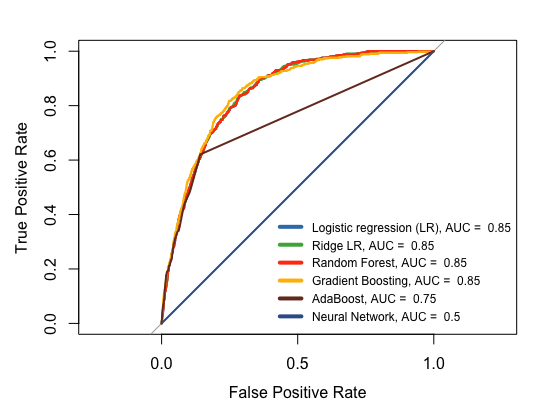
\includegraphics[width=12cm]{images/AUC_ML_opioids.png}
\caption{Predictive performance for overdose deaths had an AUC of 0.85 for three machine learning methods (logistic regression, ridge logistic regression, and random forest), but demonstrated poor performance for gradient boosting, AdaBoost, and neural network).}
\label{fig:lion}
\end{figure}

\subsection{Survival Analysis}
\begin{figure}[htp]
\centering
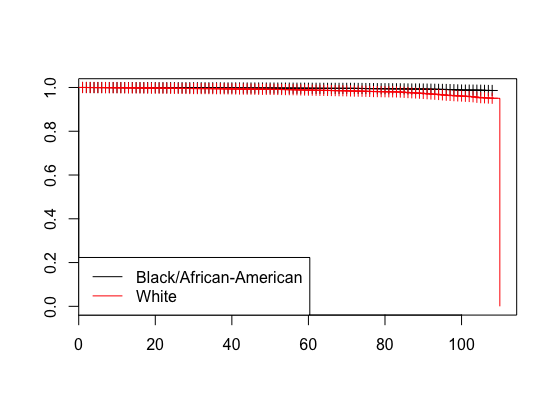
\includegraphics[width=12cm]{images/Race_KaplanMeier.png}
\caption{Kaplan Meier curve of survival indicates that }
\label{fig:lion}
\end{figure}

\begin{figure}[htp]
\centering
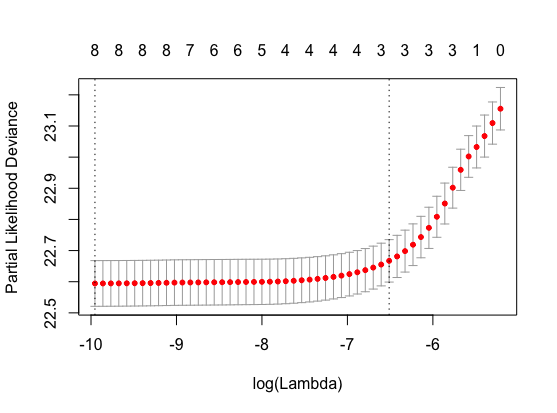
\includegraphics[width=12cm]{images/Coxmodel.png}
\caption{Cox model indicates}
\label{fig:lion}
\end{figure}

\section{Discussion and Related Work}
Significance of results
Limitations 

\section{Conclusion}

\newpage
\appendix
\section*{Appendix A.}
Some more details about those methods, so we can actually replicate them.

\newpage
\theendnotes
\bibliographystyle{ieeetr}
\bibliography{final_bibliography.bib}



\end{document} 
